\section[تمرین سوم - سوال اول: پیاده‌سازی Variational Autoencoder روی مجموعه داده CelebA]{\faSmile\ \ تمرین سوم - سوال اول: پیاده‌سازی Variational Autoencoder روی مجموعه داده CelebA}

\begin{stepbox}

\field{هدف و معرفی مسئله}{
هدف این تمرین، پیاده‌سازی گام‌به‌گام یک \lr{Variational Autoencoder (VAE)} بر روی مجموعه داده چهره‌های \lr{CelebA} بود. برای درک بهتر تفاوت میان یک اتوانکودر معمولی و نسخه واریشنال آن، ابتدا یک \lr{Simple Autoencoder} به طور کامل پیاده‌سازی و آموزش داده شد و سپس همان معماری با افزودن مکانیزم \lr{Reparameterization} و جمله \lr{KL Divergence} به یک \lr{VAE} تبدیل گردید. در پایان، عملکرد دو مدل از نظر کیفیت بازسازی تصاویر و همچنین توانایی تولید چهره‌های جدید از فضای نهفته مقایسه شد.
}

\field{آماده‌سازی داده و پیکربندی اولیه}{
مجموعه داده \lr{CelebA} با استفاده از \lr{Kaggle API} دانلود و در محیط Colab استخراج شد. با توجه به حجم بالای داده، به‌جای بارگذاری کامل تصاویر در حافظه، از کلاس \lr{ImageDataGenerator} و متد \lr{flow\_from\_directory} برای خواندن تدریجی تصاویر از روی دیسک استفاده شد. این رویکرد باعث می‌شود مصرف حافظه در طول آموزش کنترل‌شده باقی بماند، هرچند به قیمت کاهش سرعت خواندن داده از دیسک در مقایسه با نگه‌داشتن کل داده در RAM تمام می‌شود.

پارامترهای اصلی مدل مطابق خواسته سوال به شرح زیر تنظیم شدند:

\begin{itemize}
\item ابعاد ورودی تصاویر: \lr{INPUT\_DIM = (128, 128, 3)}
\item اندازه بچ: \lr{BATCH\_SIZE = 512}
\item ابعاد فضای نهفته (\lr{latent space}): \lr{Z\_DIM = 200}
\end{itemize}

مقادیر پیکسلی تصاویر نیز با ضریب \lr{1/255} نرمال‌سازی شدند تا در بازه $[0,1]$ قرار گیرند؛ این کار هم‌راستا با تابع فعال‌سازی \lr{Sigmoid} در لایه خروجی دیکودر انتخاب شده است.
}

\field{تکمیل معماری انکودر}{
انکودر متشکل از چهار لایه \lr{Conv2D} پشت‌سرهم است که هر کدام با \lr{stride=2} ابعاد مکانی تصویر را نصف می‌کنند؛ در نتیجه تصویر ورودی $128\times128\times3$ در نهایت به یک نگاشت ویژگی با ابعاد کوچک‌تر و عمق ۶۴ کانال تبدیل می‌شود. پس از هر لایه کانولوشنی از تابع فعال‌سازی \lr{LeakyReLU} استفاده شده تا از مشکل \lr{Dying ReLU} جلوگیری شود. در انتها، خروجی با \lr{Flatten} به بردار یک‌بعدی تبدیل و توسط یک لایه \lr{Dense} به بردار نهفته‌ای با طول \lr{Z\_DIM=200} نگاشت می‌شود.

خلاصه معماری (خروجی \lr{encoder.summary()}) نشان می‌دهد که تعداد پارامترهای قابل‌آموزش عمدتاً در لایه \lr{Dense} انتهایی متمرکز است؛ زیرا این لایه، خروجی مسطح‌شده با ابعاد نسبتاً بزرگ را به بردار ۲۰۰ بعدی می‌نگارد و همین موضوع سهم بزرگی از حجم کل پارامترهای مدل را به خود اختصاص می‌دهد.

\vspace{0.3cm}
\begin{center}
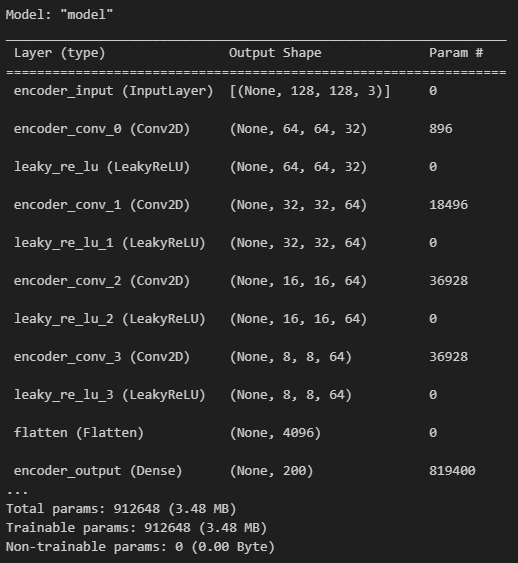
\includegraphics[width=.75\textwidth]{images/encoder_summary.png}
\captionof{figure}{خلاصه معماری انکودر اتوانکودر ساده}
\label{fig:encoder_summary}
\end{center}
}

\newpage
\field{تکمیل معماری دیکودر}{
دیکودر به‌گونه‌ای طراحی شده که تصویر آینه‌وار انکودر باشد. ابتدا بردار نهفته $200$ بعدی توسط یک لایه \lr{Dense} به همان ابعاد فضایی‌ای که پیش از \lr{Flatten} در انکودر وجود داشت (\lr{shape\_before\_flattening}) بازگردانده و با \lr{Reshape} به تانسور سه‌بعدی تبدیل می‌شود. سپس چهار لایه \lr{Conv2DTranspose} با \lr{stride=2} به‌کار رفته تا ابعاد مکانی تصویر به‌تدریج دو برابر شده و در نهایت به ابعاد اصلی $128\times128\times3$ بازگردد.

در تمام لایه‌های میانی از \lr{LeakyReLU} استفاده شده، اما لایه آخر با تابع فعال‌سازی \lr{Sigmoid} همراه شده تا خروجی مدل در بازه $[0,1]$ محدود بماند و با نرمال‌سازی انجام‌شده روی تصاویر ورودی سازگار باشد.

\vspace{0.3cm}
\begin{center}
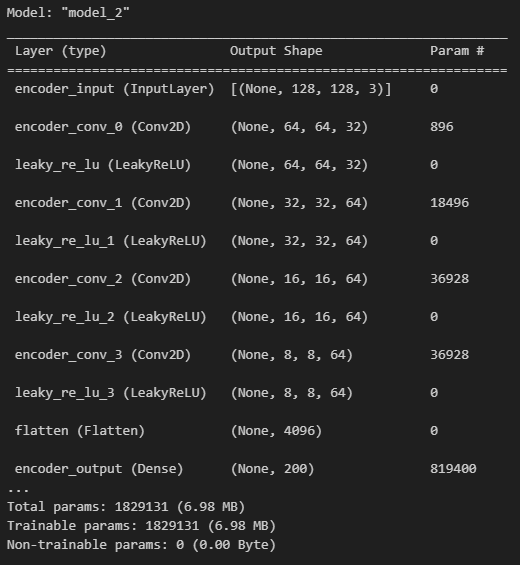
\includegraphics[width=.75\textwidth]{images/decoder_summary.png}
\captionof{figure}{خلاصه معماری دیکودر}
\label{fig:decoder_summary}
\end{center}
}

\newpage
\field{اتصال انکودر و دیکودر و آموزش اتوانکودر ساده}{
با اتصال خروجی انکودر به ورودی دیکودر، مدل کامل \lr{Simple Autoencoder} ساخته شد. ورودی مدل ترکیبی همان ورودی انکودر و خروجی آن، خروجی دیکودر است؛ یعنی مدل یاد می‌گیرد تصویر ورودی را از مسیر یک گلوگاه ۲۰۰ بعدی عبور داده و دوباره بازسازی کند.

برای آموزش، از تابع خطای \lr{Mean Squared Error} پیکسل‌به‌پیکسل به شکل زیر استفاده شد:

\[
\mathcal{L}_{r} = \frac{1}{N}\sum_{i=1}^{N}(x_i-\hat{x}_i)^2
\]

که در آن $x$ تصویر واقعی و $\hat{x}$ تصویر بازسازی‌شده توسط مدل است. بهینه‌ساز \lr{Adam} با نرخ یادگیری \lr{LEARNING\_RATE = 0.0005} به‌کار رفت و مدل به مدت \lr{N\_EPOCHS = 10} با استفاده از \lr{callback} مربوط به \lr{ModelCheckpoint} آموزش داده شد تا وزن‌های مدل پس از هر دوره ذخیره شوند.
}

\field{نتایج بازسازی تصاویر با اتوانکودر ساده}{
پس از آموزش، عملکرد مدل با مقایسه تصاویر اصلی و تصاویر بازسازی‌شده بررسی شد. همان‌طور که در شکل زیر مشاهده می‌شود، مدل توانسته ساختار کلی چهره‌ها از جمله موقعیت چشم‌ها، بینی، خطوط صورت و رنگ پوست را به‌خوبی بازتولید کند.

\vspace{0.3cm}
\begin{center}
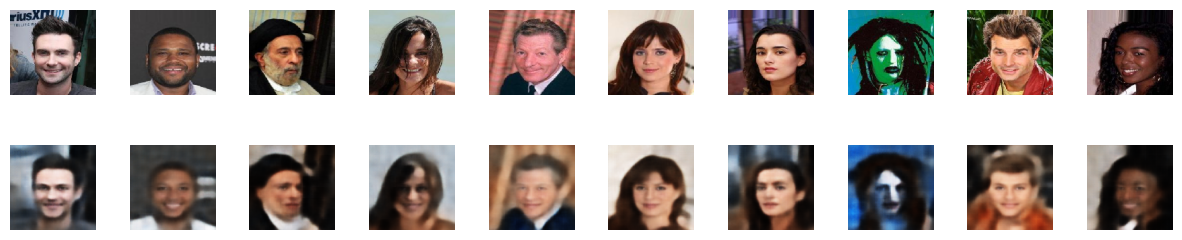
\includegraphics[width=.9\textwidth]{images/ae_reconstruction.png}
\captionof{figure}{ردیف بالا: تصاویر اصلی، ردیف پایین: تصاویر بازسازی‌شده توسط اتوانکودر ساده}
\label{fig:ae_reconstruction}
\end{center}

با این حال، تصاویر بازسازی‌شده کمی محو (\lr{blurry}) و فاقد جزئیات ریز مانند بافت مو یا لبه‌های تیز صورت هستند. این پدیده مستقیماً ناشی از انتخاب تابع خطای \lr{MSE} است؛ از آنجا که این تابع خطا، میانگین تفاوت پیکسلی را کمینه می‌کند، در حالت عدم قطعیت بین چند حالت ممکن برای یک پیکسل، مدل خروجی را به سمت میانگین آن حالت‌ها می‌برد که نتیجه‌اش محو شدن جزئیات پرفرکانس تصویر است. این محدودیت ذاتی اتوانکودرهای مبتنی بر \lr{MSE} در برابر رویکردهایی مانند \lr{GAN} که از یک شبکه تمایزدهنده برای واقعی‌تر کردن خروجی استفاده می‌کنند، به‌خوبی نمایان می‌شود.
}

\field{تبدیل به Variational Autoencoder}{
در گام بعد، انکودر بازطراحی شد تا به‌جای تولید مستقیم یک بردار نهفته قطعی، دو بردار \lr{mean\_mu} و \lr{log\_var} را تولید کند که به‌ترتیب میانگین و لگاریتم واریانس یک توزیع نرمال چندبعدی را در فضای نهفته توصیف می‌کنند. سپس با استفاده از ترفند \lr{Reparameterization Trick} نمونه‌برداری از این توزیع به شکل قابل‌مشتق‌گیری انجام شد:

\[
z = \mu + e^{\frac{1}{2}\log(\sigma^2)}\odot \epsilon \, ,\qquad \epsilon \sim \mathcal{N}(0, I)
\]

استفاده از این ترفند ضروری است، زیرا نمونه‌برداری تصادفی مستقیم غیرقابل‌مشتق‌گیری است و مانع از انتشار گرادیان در فرآیند \lr{Backpropagation} می‌شود. با انتقال تصادفی بودن به متغیر کمکی $\epsilon$، مسیر محاسباتی مربوط به $\mu$ و $\log\sigma^2$ همچنان قابل مشتق‌گیری باقی می‌ماند.

برای غنی‌تر شدن انکودر نسبت به نسخه ساده، لایه‌های \lr{BatchNormalization} و \lr{Dropout} با نرخ ۰٫۲۵ نیز به معماری افزوده شدند (\lr{use\_batch\_norm=True, use\_dropout=True}) که به تثبیت آموزش و جلوگیری از بیش‌برازش کمک می‌کنند. دیکودر بدون تغییر و دقیقاً همان دیکودر اتوانکودر ساده مورد استفاده مجدد قرار گرفت.
}

\field{تابع هزینه و آموزش VAE}{
تابع هزینه \lr{VAE} از دو جمله تشکیل شده است: جمله بازسازی (مشابه اتوانکودر ساده) و جمله \lr{KL Divergence} که فاصله توزیع نهفته تولیدشده توسط انکودر را از توزیع نرمال استاندارد $\mathcal{N}(0, I)$ اندازه می‌گیرد:

\[
\mathcal{L}_{KL} = -\frac{1}{2}\sum_{j=1}^{Z}\Big(1+\log\sigma_j^2-\mu_j^2-\sigma_j^2\Big)
\]

جمله بازسازی نیز با یک ضریب \lr{LOSS\_FACTOR = 10000} وزن‌دهی شد تا اهمیت آن در برابر جمله \lr{KL} که مقادیر کوچک‌تری دارد، حفظ شود:

\[
\mathcal{L}_{total} = \text{LOSS\_FACTOR}\times \mathcal{L}_{r} + \mathcal{L}_{KL}
\]

نقش جمله \lr{KL Divergence} این است که فضای نهفته را وادار می‌کند به‌جای پراکنده و ناپیوسته بودن (مانند اتوانکودر ساده)، حول مبدأ و به شکل یک توزیع نرمال استاندارد و پیوسته سازمان‌دهی شود. همین ویژگی است که در ادامه امکان تولید نمونه‌های جدید و معنادار را با نمونه‌برداری تصادفی از $\mathcal{N}(0, I)$ فراهم می‌کند. مدل با همان تنظیمات بهینه‌ساز \lr{Adam}، نرخ یادگیری \lr{0.0005} و به مدت \lr{10} دوره آموزش داده شد.
}

\field{نتایج بازسازی تصاویر با VAE}{
شکل زیر نتیجه بازسازی تصاویر توسط \lr{VAE} را نشان می‌دهد.

\vspace{0.3cm}
\begin{center}
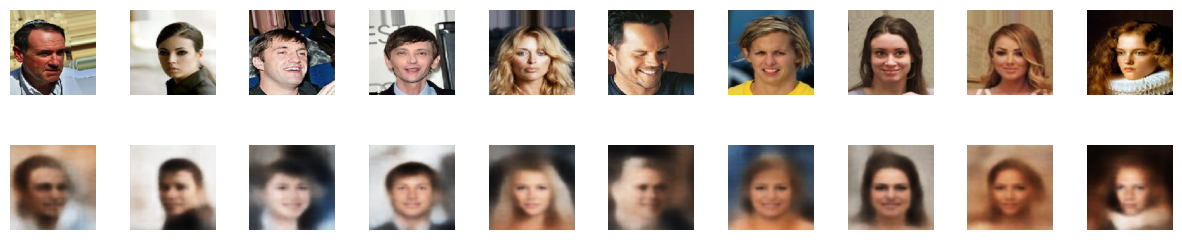
\includegraphics[width=.9\textwidth]{images/vae_reconstruction.png}
\captionof{figure}{ردیف بالا: تصاویر اصلی، ردیف پایین: تصاویر بازسازی‌شده توسط VAE}
\label{fig:vae_reconstruction}
\end{center}

در مقایسه با اتوانکودر ساده، تصاویر بازسازی‌شده توسط \lr{VAE} معمولاً اندکی محوتر به نظر می‌رسند. این موضوع طبیعی است، چرا که مدل مجبور است بخشی از ظرفیت خود را صرف برآورده‌کردن قید \lr{KL Divergence} کند، به‌جای آنکه تمام تمرکز خود را صرفاً روی کمینه‌کردن خطای بازسازی بگذارد. به بیان دیگر، بین کیفیت بازسازی و منظم‌بودن (\lr{regularity}) فضای نهفته یک \lr{trade-off} وجود دارد که با پارامتر \lr{LOSS\_FACTOR} کنترل می‌شود.
}

\field{تولید چهره‌های جدید از فضای نهفته}{
مزیت اصلی \lr{VAE} نسبت به اتوانکودر ساده، امکان تولید نمونه‌های کاملاً جدید است. با نمونه‌برداری از یک توزیع نرمال استاندارد $z\sim\mathcal{N}(0,I)$ در فضای $200$ بعدی و عبور آن از دیکودر آموزش‌دیده، تصاویری از چهره‌های جدید (که در مجموعه داده اصلی وجود نداشتند) تولید شدند.

\vspace{0.3cm}
\begin{center}
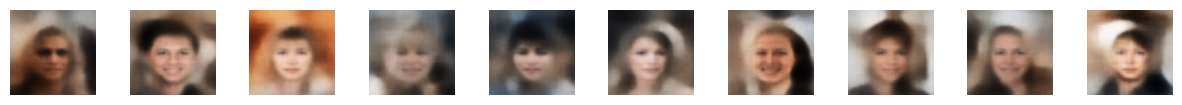
\includegraphics[width=.9\textwidth]{images/vae_generated.png}
\captionof{figure}{چهره‌های جدید تولیدشده با نمونه‌برداری تصادفی از فضای نهفته VAE}
\label{fig:vae_generated}
\end{center}

این نتیجه به‌خوبی نشان می‌دهد که به لطف جمله \lr{KL Divergence}، فضای نهفته \lr{VAE} به یک فضای پیوسته و متراکم حول مبدأ تبدیل شده که هر نقطه دلخواه در آن، به یک تصویر معنادار و شبیه به چهره انسان نگاشت می‌شود. این در حالی است که تلاش برای انجام همین کار با اتوانکودر ساده (یعنی نمونه‌برداری تصادفی از فضای نهفته آن) معمولاً به تصاویری بی‌معنا و نامفهوم منجر می‌شود؛ زیرا هیچ قیدی روی توزیع بردارهای نهفته در اتوانکودر ساده اعمال نشده و فضای نهفته آن می‌تواند خالی، ناپیوسته و پر از حفره باشد.
}

\field{مقایسه اتوانکودر ساده و VAE و اثر تغییر LOSS\_FACTOR}{
با مقایسه دو مدل می‌توان جمع‌بندی زیر را ارائه داد:

\begin{itemize}
\item از نظر کیفیت خام بازسازی (\lr{Reconstruction Quality})، اتوانکودر ساده معمولاً عملکرد اندکی بهتر و تصاویر شارپ‌تری نسبت به VAE ارائه می‌دهد، زیرا هیچ قیدی روی فضای نهفته آن اعمال نشده و تمام ظرفیت مدل صرف کمینه‌سازی خطای بازسازی می‌شود.
\item از نظر کیفیت و کاربردپذیری فضای نهفته، VAE به‌طور قطع برتری دارد، چون فضای نهفته آن پیوسته، متراکم و قابل نمونه‌برداری است و امکان تولید داده جدید (\lr{Generative capability}) را فراهم می‌کند؛ قابلیتی که اتوانکودر ساده اساساً فاقد آن است.
\item پارامتر \lr{LOSS\_FACTOR} نقش تنظیم این \lr{trade-off} را دارد: مقادیر بزرگ‌تر آن، وزن جمله بازسازی را افزایش داده و رفتار مدل را به سمت یک اتوانکودر معمولی (بازسازی شارپ‌تر، اما فضای نهفته نامنظم‌تر) سوق می‌دهد؛ در مقابل مقادیر کوچک‌تر آن، جمله \lr{KL} را پررنگ‌تر کرده و فضای نهفته را منظم‌تر می‌کند، اما به قیمت محوتر شدن بیشتر تصاویر بازسازی‌شده.
\end{itemize}

با توجه به هدف اصلی این تمرین که تولید چهره‌های جدید بود، \textbf{مدل VAE سودمندتر} از اتوانکودر ساده ارزیابی می‌شود؛ چرا که با وجود افت جزئی در وضوح بازسازی، قابلیت منحصربه‌فرد تولید نمونه‌های جدید و معنادار را در اختیار قرار می‌دهد که کاربرد اصلی و اهمیت مدل‌های مولد را نشان می‌دهد.
}

\field{جمع‌بندی}{
در این تمرین ابتدا یک اتوانکودر ساده و سپس نسخه واریشنال آن روی مجموعه داده \lr{CelebA} پیاده‌سازی و آموزش داده شد. نتایج نشان داد که هرچند اتوانکودر ساده در بازسازی تصاویر ورودی عملکرد نسبتاً خوبی دارد، اما فاقد ساختار مناسب برای تولید داده جدید است. در مقابل، \lr{VAE} با افزودن قید \lr{KL Divergence} و مکانیزم \lr{Reparameterization}، فضای نهفته‌ای منظم و پیوسته می‌سازد که امکان تولید چهره‌های جدید و باورپذیر را با نمونه‌برداری تصادفی از توزیع نرمال استاندارد فراهم می‌کند. این آزمایش به‌خوبی تفاوت بنیادین میان یک مدل فشرده‌ساز صرف (اتوانکودر ساده) و یک مدل مولد واقعی (VAE) را نشان می‌دهد.
}

\end{stepbox}